% Created by tikzDevice version 0.12.3.1 on 2021-06-16 17:28:15
% !TEX encoding = UTF-8 Unicode
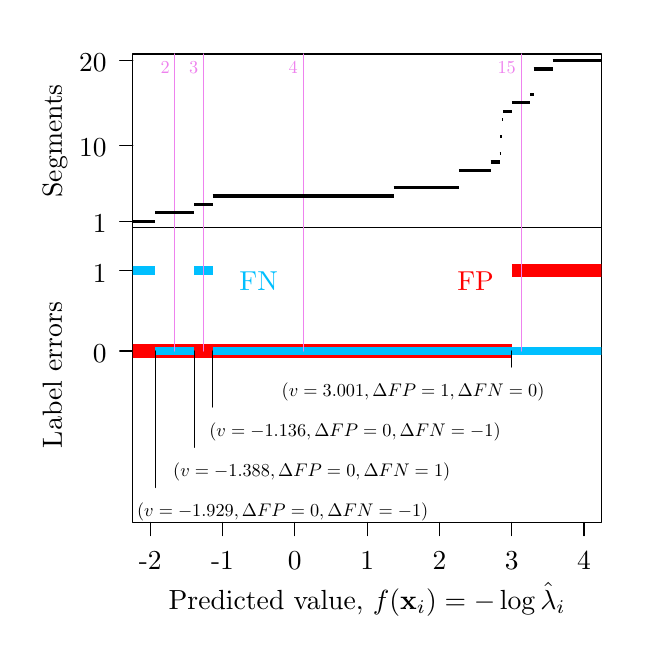
\begin{tikzpicture}[x=1pt,y=1pt]
\definecolor{fillColor}{RGB}{255,255,255}
\path[use as bounding box,fill=fillColor,fill opacity=0.00] (0,0) rectangle (216.81,216.81);
\begin{scope}
\path[clip] (  0.00,  0.00) rectangle (216.81,216.81);
\definecolor{drawColor}{RGB}{0,0,0}

\path[draw=drawColor,line width= 0.4pt,line join=round,line cap=round] ( 38.02,144.54) --
	(207.31,144.54) --
	(207.31,207.31) --
	( 38.02,207.31) --
	cycle;
\end{scope}
\begin{scope}
\path[clip] ( 38.02,144.54) rectangle (207.31,207.31);
\definecolor{drawColor}{RGB}{238,130,238}

\path[draw=drawColor,line width= 0.4pt,line join=round,line cap=round] (178.30,144.54) -- (178.30,207.31);

\path[draw=drawColor,line width= 0.4pt,line join=round,line cap=round] ( 99.52,144.54) -- ( 99.52,207.31);

\path[draw=drawColor,line width= 0.4pt,line join=round,line cap=round] ( 63.56,144.54) -- ( 63.56,207.31);

\path[draw=drawColor,line width= 0.4pt,line join=round,line cap=round] ( 53.20,144.54) -- ( 53.20,207.31);

\node[text=drawColor,anchor=base east,inner sep=0pt, outer sep=0pt, scale=  0.66] at (176.39,200.10) {15};

\node[text=drawColor,anchor=base east,inner sep=0pt, outer sep=0pt, scale=  0.66] at ( 97.62,200.10) {4};

\node[text=drawColor,anchor=base east,inner sep=0pt, outer sep=0pt, scale=  0.66] at ( 61.66,200.10) {3};

\node[text=drawColor,anchor=base east,inner sep=0pt, outer sep=0pt, scale=  0.66] at ( 51.30,200.10) {2};
\definecolor{drawColor}{RGB}{0,0,0}

\path[draw=drawColor,line width= 1.2pt,line join=round] (189.71,204.98) -- (357.79,204.98);

\path[draw=drawColor,line width= 1.2pt,line join=round] (182.78,201.92) -- (189.71,201.92);

\path[draw=drawColor,line width= 1.2pt,line join=round] (181.66,192.75) -- (182.78,192.75);

\path[draw=drawColor,line width= 1.2pt,line join=round] (174.93,189.69) -- (181.66,189.69);

\path[draw=drawColor,line width= 1.2pt,line join=round] (171.82,186.63) -- (174.93,186.63);

\path[draw=drawColor,line width= 1.2pt,line join=round] (171.46,183.57) -- (171.82,183.57);

\path[draw=drawColor,line width= 1.2pt,line join=round] (170.79,177.45) -- (171.46,177.45);

\path[draw=drawColor,line width= 1.2pt,line join=round] (170.51,171.33) -- (170.79,171.33);

\path[draw=drawColor,line width= 1.2pt,line join=round] (167.27,168.28) -- (170.51,168.28);

\path[draw=drawColor,line width= 1.2pt,line join=round] (155.80,165.22) -- (167.27,165.22);

\path[draw=drawColor,line width= 1.2pt,line join=round] (132.20,159.10) -- (155.80,159.10);

\path[draw=drawColor,line width= 1.2pt,line join=round] ( 66.85,156.04) -- (132.20,156.04);

\path[draw=drawColor,line width= 1.2pt,line join=round] ( 60.27,152.98) -- ( 66.85,152.98);

\path[draw=drawColor,line width= 1.2pt,line join=round] ( 46.13,149.92) -- ( 60.27,149.92);

\path[draw=drawColor,line width= 1.2pt,line join=round] (-112.46,146.86) -- ( 46.13,146.86);
\end{scope}
\begin{scope}
\path[clip] (  0.00,  0.00) rectangle (216.81,216.81);
\definecolor{drawColor}{RGB}{0,0,0}

\path[draw=drawColor,line width= 0.4pt,line join=round,line cap=round] ( 38.02,146.86) -- ( 38.02,204.98);

\path[draw=drawColor,line width= 0.4pt,line join=round,line cap=round] ( 38.02,146.86) -- ( 33.26,146.86);

\path[draw=drawColor,line width= 0.4pt,line join=round,line cap=round] ( 38.02,174.39) -- ( 33.26,174.39);

\path[draw=drawColor,line width= 0.4pt,line join=round,line cap=round] ( 38.02,204.98) -- ( 33.26,204.98);

\node[text=drawColor,anchor=base east,inner sep=0pt, outer sep=0pt, scale=  0.99] at ( 28.51,142.77) {1};

\node[text=drawColor,anchor=base east,inner sep=0pt, outer sep=0pt, scale=  0.99] at ( 28.51,170.30) {10};

\node[text=drawColor,anchor=base east,inner sep=0pt, outer sep=0pt, scale=  0.99] at ( 28.51,200.89) {20};

\node[text=drawColor,rotate= 90.00,anchor=base,inner sep=0pt, outer sep=0pt, scale=  1.00] at ( 12.36,175.92) {Segments};
\end{scope}
\begin{scope}
\path[clip] (  0.00,  0.00) rectangle (216.81,216.81);
\definecolor{drawColor}{RGB}{0,0,0}

\path[draw=drawColor,line width= 0.4pt,line join=round,line cap=round] ( 38.02, 38.02) --
	(207.31, 38.02) --
	(207.31,144.54) --
	( 38.02,144.54) --
	cycle;
\end{scope}
\begin{scope}
\path[clip] (  0.00,  0.00) rectangle (216.81,216.81);
\definecolor{drawColor}{RGB}{0,0,0}

\path[draw=drawColor,line width= 0.4pt,line join=round,line cap=round] ( 38.02, 99.98) -- ( 38.02,128.99);

\path[draw=drawColor,line width= 0.4pt,line join=round,line cap=round] ( 38.02, 99.98) -- ( 33.26, 99.98);

\path[draw=drawColor,line width= 0.4pt,line join=round,line cap=round] ( 38.02,128.99) -- ( 33.26,128.99);

\node[text=drawColor,anchor=base east,inner sep=0pt, outer sep=0pt, scale=  0.99] at ( 28.51, 95.89) {0};

\node[text=drawColor,anchor=base east,inner sep=0pt, outer sep=0pt, scale=  0.99] at ( 28.51,124.90) {1};
\end{scope}
\begin{scope}
\path[clip] ( 38.02, 38.02) rectangle (207.31,144.54);
\definecolor{drawColor}{RGB}{255,0,0}

\path[draw=drawColor,line width= 4.8pt,line join=round] (189.71,128.99) -- (357.79,128.99);

\path[draw=drawColor,line width= 4.8pt,line join=round] (182.78,128.99) -- (189.71,128.99);

\path[draw=drawColor,line width= 4.8pt,line join=round] (181.66,128.99) -- (182.78,128.99);

\path[draw=drawColor,line width= 4.8pt,line join=round] (174.93,128.99) -- (181.66,128.99);

\path[draw=drawColor,line width= 4.8pt,line join=round] (171.82, 99.98) -- (174.93, 99.98);

\path[draw=drawColor,line width= 4.8pt,line join=round] (171.46, 99.98) -- (171.82, 99.98);

\path[draw=drawColor,line width= 4.8pt,line join=round] (170.79, 99.98) -- (171.46, 99.98);

\path[draw=drawColor,line width= 4.8pt,line join=round] (170.51, 99.98) -- (170.79, 99.98);

\path[draw=drawColor,line width= 4.8pt,line join=round] (167.27, 99.98) -- (170.51, 99.98);

\path[draw=drawColor,line width= 4.8pt,line join=round] (155.80, 99.98) -- (167.27, 99.98);

\path[draw=drawColor,line width= 4.8pt,line join=round] (132.20, 99.98) -- (155.80, 99.98);

\path[draw=drawColor,line width= 4.8pt,line join=round] ( 66.85, 99.98) -- (132.20, 99.98);

\path[draw=drawColor,line width= 4.8pt,line join=round] ( 60.27, 99.98) -- ( 66.85, 99.98);

\path[draw=drawColor,line width= 4.8pt,line join=round] ( 46.13, 99.98) -- ( 60.27, 99.98);

\path[draw=drawColor,line width= 4.8pt,line join=round] (-112.46, 99.98) -- ( 46.13, 99.98);
\definecolor{drawColor}{RGB}{0,191,255}

\path[draw=drawColor,line width= 3.2pt,line join=round] (189.71, 99.98) -- (357.79, 99.98);

\path[draw=drawColor,line width= 3.2pt,line join=round] (182.78, 99.98) -- (189.71, 99.98);

\path[draw=drawColor,line width= 3.2pt,line join=round] (181.66, 99.98) -- (182.78, 99.98);

\path[draw=drawColor,line width= 3.2pt,line join=round] (174.93, 99.98) -- (181.66, 99.98);

\path[draw=drawColor,line width= 3.2pt,line join=round] (171.82, 99.98) -- (174.93, 99.98);

\path[draw=drawColor,line width= 3.2pt,line join=round] (171.46, 99.98) -- (171.82, 99.98);

\path[draw=drawColor,line width= 3.2pt,line join=round] (170.79, 99.98) -- (171.46, 99.98);

\path[draw=drawColor,line width= 3.2pt,line join=round] (170.51, 99.98) -- (170.79, 99.98);

\path[draw=drawColor,line width= 3.2pt,line join=round] (167.27, 99.98) -- (170.51, 99.98);

\path[draw=drawColor,line width= 3.2pt,line join=round] (155.80, 99.98) -- (167.27, 99.98);

\path[draw=drawColor,line width= 3.2pt,line join=round] (132.20, 99.98) -- (155.80, 99.98);

\path[draw=drawColor,line width= 3.2pt,line join=round] ( 66.85, 99.98) -- (132.20, 99.98);

\path[draw=drawColor,line width= 3.2pt,line join=round] ( 60.27,128.99) -- ( 66.85,128.99);

\path[draw=drawColor,line width= 3.2pt,line join=round] ( 46.13, 99.98) -- ( 60.27, 99.98);

\path[draw=drawColor,line width= 3.2pt,line join=round] (-112.46,128.99) -- ( 46.13,128.99);
\definecolor{drawColor}{RGB}{0,0,0}

\node[text=drawColor,anchor=base west,inner sep=0pt, outer sep=0pt, scale=  0.66] at ( 91.78, 83.66) {$(v=3.001,\Delta\text{FP}=1,\Delta\text{FN}=0)$};

\node[text=drawColor,anchor=base west,inner sep=0pt, outer sep=0pt, scale=  0.66] at ( 65.66, 69.15) {$(v=-1.136,\Delta\text{FP}=0,\Delta\text{FN}=-1)$};

\node[text=drawColor,anchor=base west,inner sep=0pt, outer sep=0pt, scale=  0.66] at ( 52.60, 54.65) {$(v=-1.388,\Delta\text{FP}=0,\Delta\text{FN}=1)$};

\node[text=drawColor,anchor=base west,inner sep=0pt, outer sep=0pt, scale=  0.66] at ( 39.53, 40.14) {$(v=-1.929,\Delta\text{FP}=0,\Delta\text{FN}=-1)$};
\definecolor{drawColor}{RGB}{238,130,238}

\path[draw=drawColor,line width= 0.4pt,line join=round,line cap=round] (178.30, 99.98) -- (178.30,158.00);

\path[draw=drawColor,line width= 0.4pt,line join=round,line cap=round] ( 99.52, 99.98) -- ( 99.52,158.00);

\path[draw=drawColor,line width= 0.4pt,line join=round,line cap=round] ( 63.56, 99.98) -- ( 63.56,158.00);

\path[draw=drawColor,line width= 0.4pt,line join=round,line cap=round] ( 53.20, 99.98) -- ( 53.20,158.00);
\definecolor{drawColor}{RGB}{255,0,0}

\node[text=drawColor,anchor=base,inner sep=0pt, outer sep=0pt, scale=  0.99] at (161.85,122.00) {FP};
\definecolor{drawColor}{RGB}{0,191,255}

\node[text=drawColor,anchor=base,inner sep=0pt, outer sep=0pt, scale=  0.99] at ( 83.47,122.00) {FN};
\definecolor{drawColor}{RGB}{0,0,0}

\path[draw=drawColor,line width= 0.4pt,line join=round,line cap=round] (174.93, 94.18) -- (174.93, 99.98);

\path[draw=drawColor,line width= 0.4pt,line join=round,line cap=round] ( 66.85, 79.67) -- ( 66.85, 99.98);

\path[draw=drawColor,line width= 0.4pt,line join=round,line cap=round] ( 60.27, 65.17) -- ( 60.27, 99.98);

\path[draw=drawColor,line width= 0.4pt,line join=round,line cap=round] ( 46.13, 50.66) -- ( 46.13, 99.98);
\end{scope}
\begin{scope}
\path[clip] (  0.00,  0.00) rectangle (216.81,216.81);
\definecolor{drawColor}{RGB}{0,0,0}

\node[text=drawColor,rotate= 90.00,anchor=base,inner sep=0pt, outer sep=0pt, scale=  1.00] at ( 12.36, 91.28) {Label errors};

\path[draw=drawColor,line width= 0.4pt,line join=round,line cap=round] ( 44.29, 38.02) -- (201.04, 38.02);

\path[draw=drawColor,line width= 0.4pt,line join=round,line cap=round] ( 44.29, 38.02) -- ( 44.29, 33.26);

\path[draw=drawColor,line width= 0.4pt,line join=round,line cap=round] ( 70.41, 38.02) -- ( 70.41, 33.26);

\path[draw=drawColor,line width= 0.4pt,line join=round,line cap=round] ( 96.54, 38.02) -- ( 96.54, 33.26);

\path[draw=drawColor,line width= 0.4pt,line join=round,line cap=round] (122.66, 38.02) -- (122.66, 33.26);

\path[draw=drawColor,line width= 0.4pt,line join=round,line cap=round] (148.79, 38.02) -- (148.79, 33.26);

\path[draw=drawColor,line width= 0.4pt,line join=round,line cap=round] (174.91, 38.02) -- (174.91, 33.26);

\path[draw=drawColor,line width= 0.4pt,line join=round,line cap=round] (201.04, 38.02) -- (201.04, 33.26);

\node[text=drawColor,anchor=base,inner sep=0pt, outer sep=0pt, scale=  0.99] at ( 44.29, 20.91) {-2};

\node[text=drawColor,anchor=base,inner sep=0pt, outer sep=0pt, scale=  0.99] at ( 70.41, 20.91) {-1};

\node[text=drawColor,anchor=base,inner sep=0pt, outer sep=0pt, scale=  0.99] at ( 96.54, 20.91) {0};

\node[text=drawColor,anchor=base,inner sep=0pt, outer sep=0pt, scale=  0.99] at (122.66, 20.91) {1};

\node[text=drawColor,anchor=base,inner sep=0pt, outer sep=0pt, scale=  0.99] at (148.79, 20.91) {2};

\node[text=drawColor,anchor=base,inner sep=0pt, outer sep=0pt, scale=  0.99] at (174.91, 20.91) {3};

\node[text=drawColor,anchor=base,inner sep=0pt, outer sep=0pt, scale=  0.99] at (201.04, 20.91) {4};

\node[text=drawColor,anchor=base,inner sep=0pt, outer sep=0pt, scale=  1.00] at (122.66,  6.65) {Predicted value, $f(\mathbf x_i) = -\log \hat \lambda_i$};
\end{scope}
\end{tikzpicture}
